% !TeX root = ../../tfg.tex
% !TeX encoding = utf8
%
%*******************************************************
% Construcción y evaluación de las redes neuronales 
%*******************************************************

\chapter{Construcción técnica de las redes neuronales de una sola capa}  
\label{chapter:construir-redes-neuronales}
Vista la formulación teórica de una red neuronal de una sola capa 
introducida en \ref{definition:redes_neuronales_una_capa_oculta} 
se comparará y estudiará la relación teórica 
entre nuestra propuesta de modelo y los modelos usuales de redes neuronales. 

Explicaremos también una construcción técnica junto con un
análisis del costo necesario y beneficio obtenido.
Así como los algoritmos necesarios para su evaluación y aprendizaje. 

 Los algoritmos presentados son 
 la adaptación natural de técnicas como 
\textit{forward propagation} y \textit{backpropagation } explicadas en \cite{BishopPaterRecognition} a nuestro enfoque teórico. 

Además, puesto que nuestro objetivo es optimizar seremos muy meticulosos en cuanto a analizar el 
coste computacional tanto de cómputo como de 
memoria.



\section{Componentes de una red neuronal de una capa oculta} 

Como ya habíamos definido en \ref{definition:redes_neuronales_una_capa_oculta}  
para nosotros una red neuronal será  una función $h : X \longrightarrow Y$ con $X \subseteq \R^d, Y \subseteq \R^s$ 
cuya proyección $k-$ésima viene dada por
\begin{equation}
    h_k(x) =  \sum_{i=1}^{n} \beta_{i k} \gamma_{i}( A_{i}(x))
    = 
    \sum_{i=1}^{n} \beta_{i k} \gamma_{i}
    \left(
        w_{0 i} + \sum_{j=1}^d w_{j i } x_i
    \right) 
\end{equation}
donde $n$ es el número de neuronas,   $\gamma_{i} \in \Gamma$, funciones medibles definidas de $\R$ a $\R$,
$\beta_{i k} \in \R$ y $A_i \in \afines$.

% Imagen grafo red neuronal  una capa oculta muy simple y en blanco y negro 
\begin{figure}[h!]
    \centering
    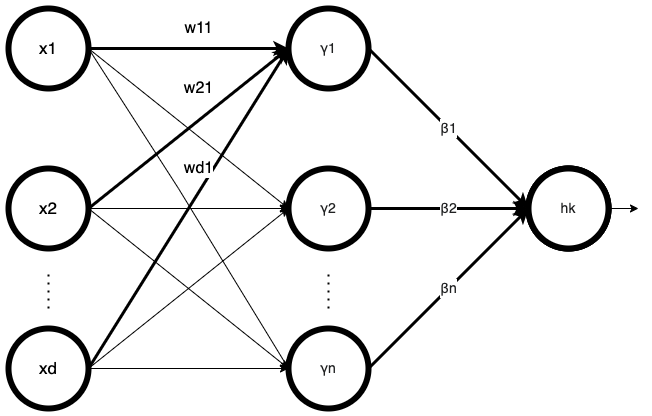
\includegraphics[width=0.85\textwidth]{1-Introduccion_redes_neuronales/Red-Neuronal-una-capa-simple.png}
    \caption{\textit{Grafo} de una red neuronal de una capa oculta}
    \label{img:grafo-red-neuronal-una-capa-oculta_repeticion}
\end{figure}

Ante esta definición el número de parámetros a ajustar es: 
\begin{itemize}
    \item De la forma $\beta_{i k}$: $n s$. 
    \item De la forma $w_{i j}$: $n(d+1)$.
\end{itemize}
Lo que hace un total de $n(s+d+1)$ parámetros, done $n$ es el número de neuronas, $s$ la dimensión de salida y $d$ la dimensión de entrada. Por lo general $d$ y $s$ son fijos ya que se suponen requisitos del problema, luego si se desea reducir el coste en memoria deberá de hacerse disminuyendo el número de neuronas.

Analizaremos más a fondo su componentes. 

\subsection*{Construcción de la primera capa}
La primera capa está compuesta por el conjunto de $n$ combinaciones
lineales del vector de entrada $(x_1, \ldots, x_d)$
a las cuales denominaremos \textit{activaciones}, $n$ será el número de sumandos definidos en \ref{definition:redes_neuronales_una_capa_oculta}  que equivale al número de neuronas en la capa oculta. 

\begin{equation}
    a_i = w_{0 i} + \sum_{i=j}^d w_{j i} x_j 
    \text{ con } j \in \{1, \ldots, n \}.
\end{equation}

Nos referiremos a los  parámetros $w_{j i}$ como 
\textit{pesos} y al parámetro $w_{0 i}$ como 
\textit{sesgo}.  

La memoria necesaria será $(d+1)n \mathfrak{F}$ 
con $\mathfrak{F}$ es el espacio requerido por un peso. 
El coste computacional es además de $d$ multiplicaciones 
y $d+1$ sumas.

\subsection*{Unidades ocultas}
Cada una de esas \textit{activaciones} será transformada
utilizando una \textit{función de activación} $\gamma_j$ 

\begin{equation}
    z_i = \gamma_i(a_i).
\end{equation}
En el contexto de las redes neuronales a $z_i$ se le conoce como \textit{unidad oculta}. Ésta  podría ser de 
nuevo  transformada por una combinación lineal, en nuestro caso tan solo 
por el producto de un escalar, ya que como se adelantó en la sección \ref{subsection:diferencia-otras-definiciones-RRNN},
 frente a la transformación afín usualmente propuesta, esta transformación no es necesaria para asegurar la convergencia, profundizaremos sobre esto más adelante. 

 Finalmente la salida vendrá dada por
 \begin{equation}
    h_k = \sum_{i=1}^n \beta_{i k} z_i 
    \text{ con } k \in \{1, \ldots, s \}.
\end{equation}
Nótese que ahora el tamaño de variables de entrada es $M$
y hay un total de $s$ unidades de activación, tanto $M$ como $s$ son
valores fijados por el diseñador de la red ya que a priori no tenemos otra información. 

 % Vamos a probar que tampoco mejora el error 
\subsection{Consideraciones sobre la irrelevancia del sesgo}
\label{consideration-irrelevancia-sesgo}
\begin{aportacionOriginal}

 Dados $X \subseteq \R^d, Y \subseteq \R^s$ y  $\Gamma$ un conjunto no vacío de funciones medibles definidas de $\R$ a $\R$, denotaremos como $\mathcal{H}^+(X,Y)$ al conjunto de redes neuronales a las cuales se le ha añadido un sesgo. 

\begin{align}
    \mathcal{H}^+(X,Y) 
    =
    \{
        h : X \longrightarrow Y 
        /& \quad 
        h_k(x) = 
        \sum_{i=1}^{n} \left( \beta_{i k} \gamma_{i}( A_{i}(x)) + \alpha_{i k} \right), \\
        & \text{donde  $h_k$  es la proyección k-ésima de $h$ con 
        $k \in \{1, \ldots, s\}$}, \\
        & n \in \N,\gamma_{i} \in \Gamma , \beta_{i k} \in \R
         \text{ y }A_{i} \text{ una aplicación afín de $\R^d$ a $\R$}           
    \}.
\end{align}


Está claro que al introducir tal sesgo se añade en memoria 
un coste de $n \mathfrak{F}$ con $n$ el número de neuronas en la capa oculta y que además el costo de cómputo se ve aumentado en la misma proporción. 
Sin embargo podría obtenerse un beneficio en cuanto a precisión, 
vamos a proceder  a analizar esta idea. 
Es evidente que 
\begin{equation} \label{eq:conjuntos-redes-neuronales-con-sesgo-contiene-elemental}
    \mathcal{H}(X,Y) \subseteq \mathcal{H}^+(X,Y)
\end{equation}

Además al estar trabajando con una sola capa, se tiene que para cualquier 
$h^+ \in \mathcal{H}^+(X,Y)$

\begin{align}
    h^+ = \sum_{i=1}^{n} \left(\beta_{i k} \gamma_{i}( A_{i}(x)) + \alpha_{i k} \right)
    = \sum_{i=1}^{n} \left(\beta_{i k} \gamma_{i}( A_{i}(x))\right) + O, 
\end{align}
con $O \in \R$ un parámetro libre.

Ante esto, al igual que se hacía en el lema \ref{lema:A_3_función_activación_continua_con_arbitaria}
es fácil obtener una neurona de valor constante y por tanto, para un conjunto fijo de neuronas $n$, se tiene que 
\begin{equation}
    \mathcal{H}^+_n(X,Y) \subsetneq  \mathcal{H}_{n+1}(X,Y),
\end{equation}
de esta relación se obtienen dos cosas: 
puesto que $n$ era arbitrario y 
\begin{equation}
    \mathcal{H}(X,Y) = \bigcup_{n \in \N} \mathcal{H}_n (X,Y)
\end{equation}
entonces como espacios de funciones 
\begin{equation}
    \mathcal{H}(X,Y) = \mathcal{H}^+ (X,Y).
\end{equation}
Por otra parte, la precisión que pueda aportar el sesgo es
superada añadiendo una neurona más a un modelo sin sesgo, es más, también se obtiene una mejora en memoria, ya que 
$\mathcal{H}^+_n(X,Y)$ requiere de $n \mathfrak{F}$ espacio de memoria adicional con respecto a $\mathcal{H}_n(X,Y)$
mientras que $\mathcal{H}_{n+1}(X,Y)$ de $(d +1) \mathfrak{F}$
y por lo visto en el teorema de convergencia universal \ref{teo:MFNAUA}, la precisión se consigue añadiendo neuronas (la dimensión de los datos es fija),
luego podemos suponer que $n$ será mayor que $d+1$. 

Hasta ahora hemos comparado la capacidad de expresión 
por la forma de los elementos de los conjuntos, para comparar su bondad aproximando, vamos a fijar  un 
 número de neuronas en la capa oculta $n$ y 
 y una función de error cualquiera que mida el error dentro 
 del conjunto de entrenamiento
 $E_{\mathcal{D}}:\mathcal{H}^+(X,Y) \longrightarrow \R^+_0$.
 
 Todas las normas en $\R^n$ son equivalentes luego no hay pérdida de generalidad fijando una cualquiera.  

 Definimos también el error dentro del espacio $\Lambda$ como 
 \begin{equation}
    \mathcal{E}_{\mathcal{D}} (\Lambda)
    = \inf \{ E_{\mathcal{D}}(h) : h \in \Lambda\}.
 \end{equation}

Está claro por la relación  
 (\refeq{eq:conjuntos-redes-neuronales-con-sesgo-contiene-elemental})
 que 
 \begin{equation}
    \mathcal{E}_{\mathcal{D}}(\mathcal{H}^+(X,Y))
    \leq
    \mathcal{E}_{\mathcal{D}}(\mathcal{H}(X,Y))
 \end{equation}

 La clave ahora reside en si se satisface la desigualdad opuesta
Es decir, dada cualquier $h^+ \in \mathcal{H}^+_n(X,Y)$ con un error de $E_D(h^+)$ existe $h \in \mathcal{H}_n(X,Y)$  tal que $E_D(h) \leq E_D(h^+).$  

Esto no es posible y para darse cuenta basta con considerar el caso de una neurona, con $G(x)$ su función de activación y $k \in \R^+$ definimos la función ideal como $f(x) = G(x) +k$. 
Tomando tan solo dos puntos convenientemente seleccionados (por ejemplo $M$ y $-M$ tal que $G(-M) = 0 y G(M) = 1$) aprecia que $H_1(\R, \R)$ no puede aproximar $f$ y sin embargo $f \in H^+_1(\R, \R)$.

% Fin de la demostración 

Concluimos tras todo esto que aunque la precisión
 que se pueda obtener con funciones de
 $\mathcal{H}_n(X,Y)$ y $\mathcal{H}^+_n(X,Y)$ es
  diferente para un mismo número de neuronas $n$,
  añadiendo una más el sesgo es irrelevante  y 
  además $\mathcal{H}^+_n(X,Y)$ tiene mayor coste
   computacional, por lo que afirmamos que 
es un artificio de las redes neuronales multicapa para enlazar una capa con otra y que en redes neuronales de una capa oculta carece de sentido.

\end{aportacionOriginal} % fin aportación original irrelevancia del sesgo


% Consideración sobre componer la red neuronal con una función
\subsection{\textit{Modus operandi} ante problemas que requieran un dominio de salida discreto}
\label{ch05:dominio-discreto}

Es usual en la literatura presentar las redes neuronales con la salida compuesta con una función $\theta$, de tal manera que una red neuronal sea de la forma

\begin{equation}\label{red-neuronal-con-compuesta}
    h_k(x) = \theta_k 
    \left(
        \sum_{i=1}^{n} \beta_{i k} \gamma_{i}
    \left(
        w_{0 i} + \sum_{j=1}^d w_{j i } x_i
    \right) 
    \right)
    \text{ para cada  } k \in \{1, \ldots, s \}.
\end{equation}
El teorema universal de convergencia \ref{teo:MFNAUA} nos asegura 
que dado un número lo suficientemente grande de neuronas tal 
composición no es necesaria. Sin embargo, a nivel práctico ese 
número de neuronas puede no alcanzarse y, por cómo se produce la convergencia, el resultado serán funciones con imágenes con forma de dominios contenidos en $\R^n$.

Por la naturaleza de la imagen de ciertos problemas no sería 
necesaria mayor modificación y con nuestra definición sería 
más que suficiente. Pero en caso de que la salida tenga que cumplir alguna restricción, como por ejemplo en 
problemas de clasificación que necesiten de una salida discreta; sería necesario la composición con una función 
$\theta$ que discretice la imagen como observábamos en \ref{corolario:2_5_función_Booleana}.  


La situación por tanto es la siguiente, si procedemos como en \refeq{red-neuronal-con-compuesta}, se tendría que si $f$ es el patrón subyacente de la clasificación y $\theta$ la función que discretiza el dominio se deberá de encontrar 
$h \in \rrnnmc$ tal que $h$ aproxime a $\theta^{-1} \circ f$.

Lo cual exige que $\theta$ tenga inversa y que sea medible, además de la cuestión de qué $\theta$ es la más conveniente $\dots$

\begin{aportacionOriginal} % aportación original salida discreta
    
Es por ello que en nuestra aproximación descartamos este modo de proceder y proponemos el siguiente: 

\begin{enumerate}
    \item Entrenamos $h\in \rrnnmc$, esto dará una salida que no necesariamente será discreta. 
    \item Una vez que se ha calculado $h$,  $\theta$ se determina a partir de $h$. 
\end{enumerate}

\subsubsection*{Construcción de  $\theta$}

Una vez fijada $h$,  para $A \subseteq \mathcal{D}$ se define  el conjunto 
\begin{equation}
    \Lambda = \{(h(x), y) : (x,y) \in A\}.
\end{equation}

A partir del cual $\theta$ será una función que se ha obtenido por el método de clasificación supervisada de los $k$-vecinos más cercanos ($k-$NN) donde el conjunto de entrenamiento es $\Lambda$.

El motivo por el que se ha optado por esta aproximación es que si consideráramos $\theta$ como una función a trozos usual definida como 

\begin{equation}
    \tilde{\theta}(x) = y \text{ si } h(x) \in I_y.
\end{equation}

Donde $I_y$ puede no ser un intervalo conexo y que introduciría complejidad al cálculo y determinación de $\tilde{\theta}$, es por ello que lo natural sería entonces construir un función que discretice a partir de los valores conocidos más cercanos, esto es el algoritmo $k-$NN.  

\end{aportacionOriginal}  % aportación original salida discreta

\subsubsection*{Construcción de $k-$NN}  

Si la dimensión de salida con la que se ha entrenado $h$ es uno, es decir $s=1$. Por ser $\R$ de una dimensión lo natural sería hacer $k=1$, es decir 

\begin{align}
    & \theta(h(x)) = y_{cercano}, \\
    &\text{donde } 
    (h(a),  y_{cercano}) \in A 
    \text{ y }
    h(a) = \min \{|h(x) - h(b)| :  (h(b),  y) \in A  \}.
\end{align}

La implementación de la fórmula anterior sería la siguiente: 

% Algoritmo 1-NN
\begin{algorithm}[H]
   \caption{ Cálculo de la función $\theta$ como clasificador $1-$NN} 
   \textbf{Input: } Conjunto de datos $\Lambda$.  \\
   \textbf{Output: } Función $\theta : \R \longrightarrow \R$
   \begin{algorithmic}[1]
    \STATE \COMMENT{Definimos $\theta$ como} \\
    \SetKwFunction{FSum}{$\theta$}
    \SetKwProg{Fn}{Function}{:}{}
    \Fn{\FSum{$h_x$}}{
        \STATE \textit{distancia mínima} $\gets\infty$
        \STATE $clase \leftarrow NADA$ \\
        \STATE \COMMENT{Encontramos el más cercano}\\
        \ForAll{cada $(h, y)$}{
            \If{$distancia(h,h_x) <$\textit{distancia mínima}}{
               $clase \leftarrow y$
            }
        }
        \Return{$clase$}
    } 
    \Return{$\theta$}
   \end{algorithmic}
\end{algorithm}

%%%%%%%%%%% Fin de lo observado

\subsection{Qué función de activación seleccionar}

Los aspectos a tener en cuenta a la hora de seleccionar una función 
de activación frente a otra de una red neuronal serían los siguientes:
\begin{enumerate}
    \item Espacio de memoria.
    \item Coste computacional.
    \item Efectividad en cuanto a reducir el error de aproximación.
\end{enumerate}

Sobre la primera consideración está claro que el uso de una única función ahorraría el tener que almacenar el tipo de función que se va emplear en cada neurona.

Respecto al coste computacional puede uno basarse en una análisis teórico del número de 
operaciones y su complejidad o realizar un estudio empírico se ha realizado 
en al sección \ref{ch06:coste-computacional-funciones-activacion}.

% Nota margen sobre idea 
\marginpar{\maginLetterSize
    \iconoClave \textcolor{darkRed}{     
        \textbf{
        Estrategia de selección de funciones de activación.
        }
    }

    Esta idea abre la puerta a determinar mediante algoritmos 
    de optimización qué funciones de activación podrían resultar más 
    beneficiosas.
    Ideas similares usando algoritmos genéticos 
    se encuentra en artículos como 
    \cite{FunctionOptimizationwithGeneticAlgorithms}
    y 
    \cite{Genetic-deep-neural-networks}
    sin embargo expondremos nuestra versión en el capítulo 
    \ref{ch08:genetic-selection}.
    
}
Fijado cierto número de neuronas, en lo que respecta a la precisión que nos puedan aportar las funciones de activación; por la idea intuitiva 
del funcionamiento de las funciones de activación mostrado en mostrada en \ref{ch03:funcionamiento-intuitivo-funcion-activacion} es un factor que repercute en los resultados 
pero desconocido a priori. 


%% Formulación técnica 

\section{Construcción explícita y evaluación de una red neuronal}

Ante todas las consideraciones expuestas y puesto que 
no existe ningún resultado o hipótesis a favor de combinar funciones de activación, en pos de simplificar el estudio, vamos a suponer a priori que todos los nodos están compuestos con la misma. Entonces,  una red neuronal para nosotros 
vendrá determinada dos matrices de pesos y una función de evaluación. 

Es decir siguiendo la idea constructiva expuesta en manuales tales como \cite{learning-from-data-1-2}
 cualquier $h \in \rrnnsmn$ de $n$ neuronas en la capa oculta se implementa como 
$(\gamma, M_{n \times (1+r)}, M_{(n+1) \times s})$ con $M_{f \times c}$ matrices de dimensiones $f$ filas y $c$ columnas. 

$\gamma$ representa a función de activación en cada nodo. 
$M_{n \times (1+r)}$ son los pesos de la primera capa 
y $M_{(n+1) \times s}$ son los pesos de la salida. 

Tomando como $\mathfrak{I}_{r+1}: \R^r \longrightarrow M_{(r+1) \times 1}(\R)$ a la aplicación inyección que a cada vector $(x_1, \ldots, x_d)$ le hace corresponder el vector columna $(1, x_1, \ldots x_d)^T.$
Además entendemos para una función $\gamma : \R \longrightarrow \R$ 
que la imagen de la composición de una matriz con $\gamma$ es evaluar cada una de sus entradas por $\gamma$. 
Con esta representación evaluar una red neuronal consistiría en el producto matricial de 

\begin{equation}
    h(x) =  M_{(n+1) \times s} \cdot
    \mathfrak{I}_{n+1}\left(
         \gamma \left( 
             M_{n \times (1+d)} 
            \cdot 
            \mathfrak{I}_{d+1}(x)
        \right)
    \right).
\end{equation}

El coste computacional de tal operación es 
\begin{table}[h]
    \begin{center}
    \begin{tabular}{| c | c |}
    \hline
    Operación & Apariciones  \\ \hline
    $+$ & $n d+n s = n(d+s)$  \\
    $\times$ & $n(d+1)+(n+1)s = n(d+s+2)$  \\
    $\gamma$ & $n$  \\
    $\mathfrak{I}$ & $2$  \\
    \hline
    \end{tabular}
    \caption{Coste computacional de la implementación propuesta en \cite{MostafaLearningFromData}}
    \label{tab:coste computacional de la implementación de Mustafa}
    \end{center}
\end{table}

\subsection*{Primera optimización reformulando la implementación de una red neuronal}

Sin embargo de acorde a nuestro modelo definido en \ref{definition:redes_neuronales_una_capa_oculta}, nuestra propuesta de representación es al siguiente: 

\begin{equation}
    (\gamma, A, S, B) 
    \text{ donde } 
    A \in M_{n \times d}(\R), 
    S\in M_{n \times 1}(\R) 
    \text{ y }
    B \in M_{s \times n}(\R).
\end{equation}
y con esta representación la evaluación sería

\begin{equation}
    h(x) =  B \cdot
        \gamma \left( 
            A
            \cdot 
            x
            + S
        \right),
\end{equation}
que tiene un coste computacional de 
\begin{table}[h]
    \begin{center}
    \begin{tabular}{| c | c |}
    \hline
    Operación & Apariciones  \\ \hline
    $+$ & $n d+n(s-1) = n(d+s-1)$  \\
    $\times$ & $n d+n s = n(d+s)$  \\
    $\gamma$ & $n$  \\
    $\mathfrak{I}$ & $0$  \\
    \hline
    \end{tabular}
    \caption{Coste computacional de nuestra implementación de red neuronal de una capa}
    \label{tab:coste computacional nuestr modelo red neuronal}
    \end{center}
\end{table}

Que como vemos ha supuesto una mejora de 

\begin{table}[h]
    \centering
    \resizebox{\textwidth}{!}{
        \begin{tabular}{| c | c | c | c |}
        \hline
        % cabecera 
        Operación 
        & Coste formulación usual \ref{tab:coste computacional de la implementación de Mustafa}
        & Coste nuestra propuesta \ref{tab:coste computacional nuestr modelo red neuronal} 
        & Operaciones reducidas  \\ \hline
        $+$ & $n(d+s)$ & $n(d+s-1)$ & $n$\\
        $\times$ & $n(d+s+2)$ & $n(d+s)$  & $2n$\\
        $\gamma$ & $n$  & $n$  & $0$ \\
        $\mathfrak{I}$  & $2$ & $0$ & $2$ \\
        \hline
        \end{tabular}
    }
    \caption{Comparativas de coste computacional entre la implementación usual de una red neuronal y la nuestra}
    \label{tab:comparativas coste red neuronal }
\end{table}

Además se ha reducido el espacio de memoria en $n$ unidades del tipo de datos que utilicen las redes neuronales. 

\subsubsection*{Ejemplo de evaluación de una red neuronal}

\begin{figure}[h!]
    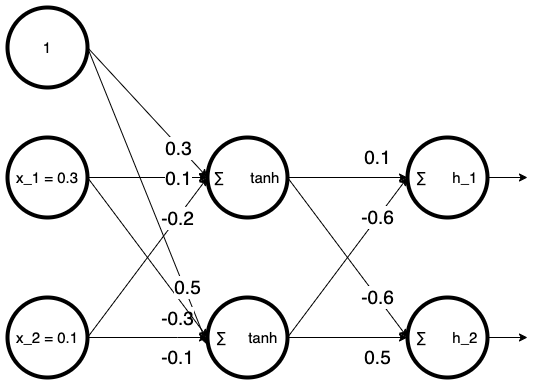
\includegraphics[width=0.7\textwidth]{4-Actualizacion_redes_neuronales/evaluacion-1-capa.drawio.png}
    \centering
    \caption{Ejemplo de evaluación de una red neuronal de una capa con entrada y salida de tamaño dos y dos neuronas en la capa oculta}
    \label{img:Ejemplo-evaluación-red-neruonal-una-capa}
\end{figure}

A continuación vamos a dar un ejemplo basado en la red neuronal mostrada en la imagen \ref{img:Ejemplo-evaluación-red-neruonal-una-capa}, 
La red neuronal viene dada por las matrices: 
la matriz de la primera capa asociada es 
\begin{equation}
     A = 
        \begin{bmatrix}
            0.1 & -0.2 \\
            -0.3 & -0.1 
        \end{bmatrix}  
\end{equation}
la matriz de sesgos 
\begin{equation}
    S = 
        \begin{bmatrix}
            0.3  \\
            0.5 
        \end{bmatrix}  
\end{equation}
La matriz de pesos de la capa oculta sería 
\begin{equation}
     B = 
    \begin{bmatrix}
        0.1 & -0.6 \\
        -0.6 & 0.5
    \end{bmatrix}. 
\end{equation}

Para la entrada  $x = (0.3, 0.1)$ los sucesivos cálculos serían
\begin{equation}
    A x = 
    \begin{bmatrix}
        0.1 & -0.2 \\
        -0.3 & -0.1 
    \end{bmatrix}  
    \begin{bmatrix}
        0.3  \\
        0.1 
    \end{bmatrix}
    = 
    \begin{bmatrix}
        0.01  \\
        -0.1 
    \end{bmatrix}
    . 
\end{equation}

\begin{equation}
    A x +S= 
    \begin{bmatrix}
        0.01  \\
        -0.1 
    \end{bmatrix}
    + 
    \begin{bmatrix}
        0.3  \\
        0.5 
    \end{bmatrix}
    = 
    \begin{bmatrix}
        0.31  \\
        0.4 
    \end{bmatrix}
    . 
\end{equation}

\begin{equation}
    \gamma (A x +S) = 
    \gamma \left(
    \begin{bmatrix}
        0.31  \\
        0.4 
    \end{bmatrix}
    \right)
    = 
    \begin{bmatrix}
        \gamma(0.31)  \\
        \gamma(0.4) 
    \end{bmatrix}
    = 
    \begin{bmatrix}
        0.3004 \\
        0.3799  \\
    \end{bmatrix}.
\end{equation}

Finalmente las respectivas salidas de las capas ocultas serían
\begin{equation}
    B  \gamma (A x +S)  
    = 
    \begin{bmatrix}
        0.1 & -0.6 \\
        -0.6 & 0.5
    \end{bmatrix}
    \begin{bmatrix}
        0.3004 \\
        0.3799  \\
    \end{bmatrix}
    = 
    \begin{bmatrix}
        -0.1979 \\
       0.0097  \\
    \end{bmatrix}.
\end{equation}

\subsection{Implementación de una red neuronal y evaluación}
\label{section:rrnn_implementation}
Como conclusión a todo lo explicado una red neuronal no 
sería más que una estructura que almacenara $(\gamma, A, S, B)$, esto es 

% Pseudo código que refleja la estructura de una red neuronal 

\begin{algorithm}[H]
    \caption{Estructura de una red neuronal}
    \label{algoritmo:estructura de una red neuronal}
    \DontPrintSemicolon
    \hspace*{\algorithmicindent} 
        \textbf{Entrada}:
        \begin{itemize}
            \item $d$: Dimensión de los datos de entrada.
            \item $s$: Dimensión que define una red neuronal.
            \item $n$: Número de nodos en la capa oculta. 

        \end{itemize}
        \hspace{\algorithmicindent} 
        \Struct{Red neuronal(d,s,n)}{
            $A \gets$ Matriz $n$ filas $d$ columnas\;
            $S \gets$ Matriz $n$ filas $1$ columnas\;
            $B \gets$ Matriz $s$ filas $n$ columnas\;
        }
        \hspace{\algorithmicindent} 
  \end{algorithm}

y si quisiéramos evaluar la red neuronal el algoritmo sería el siguiente 
  %% Algoritmo de evaluación de redes neuronales 

  \begin{algorithm}[H]
    \caption{Evaluación de una red neuronal, \textit{Forward propagation}}
    \label{algoritmo:evaluar red neuronal}

    \hspace*{\algorithmicindent} 
        \textbf{Entrada}:
        \begin{itemize}
            \item $x$: Vector de atributos que se desea evaluar con la red neuronal.
            \item $h = (\gamma, A, S, B)$ representa la red neuronal que se desea evaluar y la función de activación $\gamma$ con la que se va a evaluar. 
        \end{itemize}
        \hspace{\algorithmicindent} 
        \SetKwFunction{Main}{ForwardPropagation}
        \SetKwProg{F}{Function}{:}{}
        \F{\Main{$h, x$}}{ 

            $sensibilidad \gets A \cdot x + S$ \;
            $primeraCapa \gets$ Se crea vector del mismo tamaño que $sensibilidad$ \;
            \ForEach{ entrada-Iésima-Neurona $\in$ sensibilidad}{
                $primeraCapa[i] \gets \gamma($ entrada-Iésima-Neurona $)$
            }
            \;
            $salida \gets B \cdot primeraCapa$ \;
            \KwRet $salida$ \;
        }
  \end{algorithm}
  \newpage






